When describing rotating particles it is common to use the so called Euler Angles. These are defined 

DEFINITION OF EULER ANGLES

This is illustrated in figure \ref{fig:eulerangles} where each prim marks one more step of rotation to the coordinate system of

\begin{figure}
\begin{center}
\includegraphics[width=0.7\textwidth]{figures/theory/eulerangles.png}
\end{center}
\caption{The Euler angles illustrated using a series of coordinate rotations. This is the normal way of illustrating the Euler angles as it is how they are defined.}
\label{fig:eulerangles}
\end{figure}


\begin{figure}
\begin{center}
\includegraphics[width=0.7\textwidth]{figures/theory/EulerAngles.png}
\end{center}
\caption{The Euler angles illustrated using an ellipsoid. This alternate visualization shows the angles with a point of view similar to that of the camera in the experiment. Note although $\psi$ has an impact on the particle dynamics, as the particle is nearly axis-symmetric we can not observe it}
\label{fig:eulerparticle}
\end{figure}


